\documentclass[pagesize=auto,bibliography=totocnumbered]{scrbook}

\title{Learn to Code in C\#: An Introduction with Media Computation}
\author{Dr Michael James Scott} % Author

\usepackage{ifpdf}
\usepackage{tikz,pgfplots}
\usepackage{amsmath}
\usepackage{minted}
\usepackage{hyperref}
\pgfplotsset{compat=1.18}
\usepgfplotslibrary{external}
\tikzexternalize[
    prefix={images/tikz/}
]

\ifpdf
\tikzset{
    export as svg/.style={
        external/system call/.add={}{
            && pdf2svg "\image.pdf" "\image.svg"
%            && magick convert -density #1 -transparent white "\image.pdf" "\image.png" && ebb -x "\image.png"
        },
%        /pgf/images/external info, /pgf/images/include external/.code={ \setlength{\fboxrule}{0pt} \fbox{\includegraphics[scale=.24]{##1.png}} }
    },
    export as png/.default={144},
}
\tikzset{export as svg}
\else 
\pgfkeys{/pgf/images/include external/.code={ \includegraphics{#1.svg} } }
\fi

\immediate\write18{if not exist tikz_external mkdir images/tikz}

\ifdefined\HCode
  \def\pgfsysdriver{pgfsys-dvisvgm4ht.def}
\fi 

\colorlet{LightGray}{gray!5}


\usepackage{xspace}
\usepackage{hyphenat}
\hyphenation{}

% Provide full error messages
\errorcontextlines 10000

% Enables checking if XeLaTeX is used.
\usepackage{ifxetex}

% Load additional packages for the PDF output
\ifxetex
	% adjusting figures to fit into the width of a page.
	\usepackage{adjustbox}
    
	% Fancy lines for chapters and end of sections.
	\usepackage{psvectorian}
\else
	% Ignore adjustbox commands (HTML files do not have a width).
	\newcommand{\adjustbox}[2][]{#1}

	% Ignore psvectorian lines.
	\newcommand{\psvectorian}[2][]{}

\fi

% Translate horizontal rule and emdash into hrule / "---"
\ifx\HCode\undefined 
	\def\myrule{\hrule}
	\newcommand{\emdash}[1][]{\hspace{0pt}---\hspace{0pt}}
	\newcommand\nextpage[1][]{\newpage}      
\else
	\def\myrule{\HCode{<hr style="clear: both" />}}
	\def\emdash{\HCode{&\#8212;}}
    \newcommand\nextpage[1][]{\HCode{<mbp:pagebreak />}}
\fi

% load packages
% Set up bibliography.

% Advanced handling of quotation marks -> important for bibliography.
\usepackage{csquotes}

%load babel
\usepackage[american]{babel}

\ifxetex
% See https://www.ctan.org/pkg/biblatex for documentation.
	\usepackage[indexing=cite,style=authoryear,natbib=true]{biblatex}
	\addbibresource{bibliography/references.bib}
\else
	\usepackage{natbib}
	\usepackage{usebib}
	\bibinput{bibliography/references}

	% \citetitle does not work with natbib / pdfLaTeX -> translate into \usebibentry
	\newcommand{\citetitle}[2][]{\textit{\usebibentry{#2}{title}}}
\fi

% Set bibliography to footnote size
\renewcommand{\bibfont}{\footnotesize}

\newcommand{\bibpreface}[1]{\patchcmd{\thebibliography}{\list}{#1\list}{}{}}

% Write the name of a referenced section or chapter label with \nameref{label}.
\usepackage{nameref}
% for ebook and web
\usepackage[paperwidth=5.25in,  paperheight=8in, inner=0.80in, outer=0.3in, top=0.7in, bottom=0.5in]{geometry}



\usepackage{idxlayout}
% prevent splitting footnotes over several pages, see https://texfaq.org/FAQ-splitfoot
\interfootnotelinepenalty=10000

% Set line separator between items in an itemize environment to 5pt 
\usepackage{enumitem}
\setlist[itemize]{parsep=5pt}

% Set the space between paragraphs and deactivate indentation for paragraphs
\setlength{\parskip}{1.4\baselineskip}
\setlength{\parindent}{0pt}

% Set font size of captions to small, the font size of index to very small, and the footnote font size to very small.
%\usepackage[labelfont=bf]{caption}
%\captionsetup{font=small}
\usepackage{imakeidx}
\indexsetup{othercode=\footnotesize}
\renewcommand{\footnotesize}{\scriptsize}

% you can use ``same'' (same font as your document's), ``sf'', ``tt''  or ``rm'' for monospaced font, also see https://www.ctan.org/pkg/url
\usepackage{url}
\urlstyle{same}

% Font tweaks not available for e-books.
\ifxetex

% Slightly tweak font spacing for aesthetics.
	\usepackage{microtype}
	\usepackage{lmodern}

% Use Linux Libertine font. For other fonts, check out http://www.tug.dk/FontCatalogue/
	\usepackage{libertine}
\else
\fi


% prefer more spaces between words rather than more hyphenations at the end of a line
\sloppy

\begin{document}
\frontmatter

% front matter chapter entries use roman page numbering (i, ii, iii, iv, ...)
\pagenumbering{roman}

%%%%%%%%%%%%%%%%%%%%%%%%%%%%%%%%%%%%%
% Read the /ReadMeFirst/ReadMeFirst.tex for an introduction. Check out the accompanying book "Better Books with LaTeX the Agile Way" for a discussion of the template and step-by-step instructions. The template was originally created by Clemens Lode, LODE Publishing (www.lode.de), mail@lode.de, 8/17/2018. Feel free to use this template for your book project!
%%%%%%%%%%%%%%%%%%%%%%%%%%%%%%%%%%%%%

\thispagestyle{empty}

% Replace "Replace with your Title" with your book title
% Replace "Replace with your subtitle" with your book subtitle
% Replace "Publishing Company, Location" with your company's name and location 
% Upload a low res jpg and a high res png version of your front cover into the "images" folder
% Replace "bover_highres.png" and "bover.jpg" with your file name

\vspace{3cm}
  \begin{center}
	\bfseries \sffamily \Huge Learn to Code in C\# \par
	\bfseries \LARGE An Introduction with Media Computation \par
~\\
	
    \ifpdf
		\includegraphics[width=0.65\textwidth]{images/cover.jpg}

	\else
		\href{learn2codech1.html}{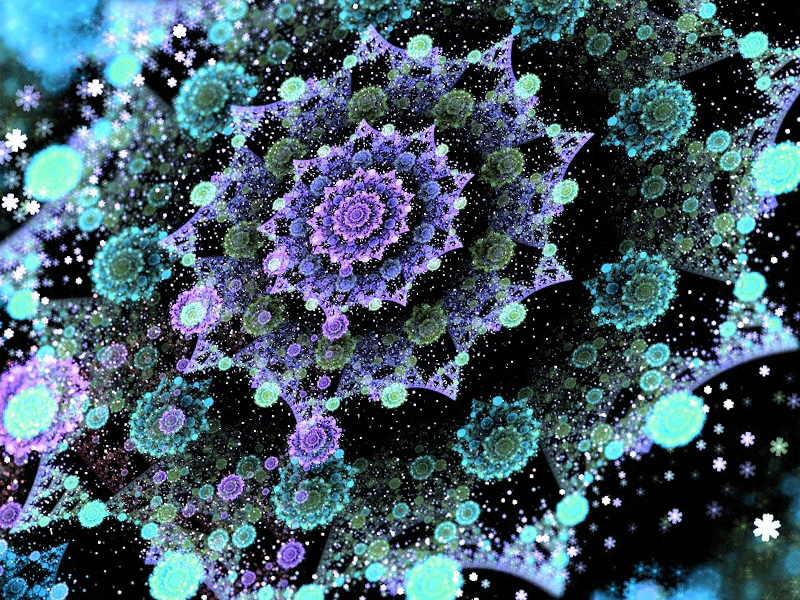
\includegraphics{images/cover_web.jpg}}
    \fi
    
	~\\
	\bfseries \small Dr Michael James Scott\par
  \end{center}

\newpage

%%%%%%%%%%%%%%%%%%%%%%%%%%%%%%%%%%%%%
% Read the /ReadMeFirst/ReadMeFirst.tex for an introduction. Check out the accompanying book "Better Books with LaTeX the Agile Way" for a discussion of the template and step-by-step instructions. The template was originally created by Clemens Lode, LODE Publishing (www.lode.de), mail@lode.de, 8/17/2018. Feel free to use this template for your book project!
%%%%%%%%%%%%%%%%%%%%%%%%%%%%%%%%%%%%%

% Replace Your company's name with your company's name.
% Replace Your company's location (city) with your company's location.
% Replace Your website's URL with your website's URL.
% Replace Your email address with your email address.
% Replace Edition with the edition number.
% Replace ISBN with your ISBN. 
% Replace Your editor's name with your editor's name.
% Replace Your designer's name with your book cover designer's name.
% Add your image sources and icons including the license.
% Replace Your newsletter email with your newsletter email.
% Replace Your website's URL with your website's URL.


\thispagestyle{empty}
\begin{center}

\copyright~\the\year~\textit{Ninja Nyan Ltd}, Penryn, Cornwall\\
\textsc{All Rights Reserved.}\\
%\url{Your-website's-URL}
	~\\
For more information about permission to reproduce selections from this book, please contact the author.

\ifpdf
	~\\\par
	\the\year~Edition
\else
	~\\
	E-book created \today
\fi

% Impression line, indicating number and year of current printing
% International Standard Book Number (ISBN)
% International Standard Serial Number (ISSN), if applicable
\ifpdf
	~\\
	\textsc{ISBN 978-3-16-148410-0}
\fi

% For translations, indication of original-language title, publisher, and copyright, acknowledgments, permissions, and other credits, including acknowledgment of grants, if applicable and space permitting

%Edited by: \emph{Eve Scott}\\
%Cover design: \emph{Phoebe Herring}\\
%Image sources: \emph{Your image sources, e.g., shutterstock}\\


%Paper durability statement
\ifxetex
	~\\
	Printed on acid\hyp{}free, unbleached paper.
\fi

%Subscribe to our newsletter. Simply write to \url{Your-newsletter-email} or visit our website \url{Your-website's-URL}.

%\ifxetex
%\else
	~\\	
	\textit{This version licensed for use in education only.}
	%\myrule
%\fi
	
\end{center}



% Also check out http://www.chicagomanualofstyle.org/16/ch01/ch01_sec019.html\newpage

%\input{lib/tableofcontents}\newpage

\renewcommand*{\chapterpagestyle}{plain}

\mainmatter

% reset to normal page numbering (1, 2, 3, ...)
\pagenumbering{arabic}

\foreach \x in {1,...,3} {
     \input{chapters/\x}\newpage
 }

\end{document}
